
\documentclass[a4paper,11pt]{article}

% * Activating Greek fonts in Latex
  \usepackage[english,greek]{babel} % the last language is the default

%enum greek letters
 \usepackage{moreenum}
 
 
 \usepackage{multirow}


  \newcommand{\lt}{\latintext}
  \newcommand{\gt}{\greektext}


% * Math packages
 % \usepackage{amsthm}
  \usepackage{amsmath}
 % \usepackage{amssymb}
    
% * graphics package
  \usepackage{graphicx} 

% * verbatim writing package (mainly used to import program's code)
  \usepackage{verbatim}

% ------------------------------------------------------------------------------- %


% ------------------------------------------------------------------------------- %
% Here we set the title, the author and the date of our document.
%
% * Setting the title of the document
  \title{\textbf{Προαιρετική Εργασία στο Μάθημα της Αριθμητικής Ανάλυσης}} % Put your own title here

% * Setting the author or authors of the document
  \author{Όνοματεπώνυμο: Γεώργιος Δάλλας  \\  ΑΕΜ: 4116}       % Put your own Name and AEM here

% * Setting the date of the document
  \date{\today}                                      % Put a specific date here
% ------------------------------------------------------------------------------- %


% =============================================================================== %
% ||                       HERE WE BEGIN OUR DOCUMENT                          || %
% =============================================================================== %
\begin{document}

% *** We are now inside the document everything from now on is VISIBLE!!! *** %

% Command that prints the title of your document
\maketitle

\section{Πρώτη άσκηση}
\begin{center}  

{\scriptsize Α}{\footnotesize Β}{\small Γ}{\normalsize Δ}{\large Ε}{\Large Ζ}{\LARGE Η}{\huge Θ}{\Huge Ι}{\huge κ}{\LARGE λ}{\Large μ}{\large ν}{\normalsize ξ}{\small ο}{\footnotesize π}{\scriptsize ρ}{\tiny σ}

\end{center}
\section{Δεύτερη άσκηση}
\begin{center}\lt
Normal \textit{Italics} \textbf{Bold}\\
\emph{Emphasized} \underline{Underlined}
\end{center}\gt
\section{Τρίτη άσκηση}\lt
\begin{center}
$a^2+b^2=c^2$\\
$e^{i\pi}=-1$\\
$\pi = \dfrac{c}{d}$\\
$\dfrac{d}{dx} \int_{a}^{x}f(s)ds=f(x)$\\
\[f(x)=\sum_{i=0}^{\infty}\dfrac{f^{(i)}(0)}{i!}x^i\]
$\textbf{Ax=b}$\\
$\|x+y\| \leq \|x\|+\|y\| $\\

\begin{equation}
\textbf{I}=\begin{pmatrix}    
    1 & 0 & 0 & 0 \\ 
    0 & 1 & 0 & 0 \\
    0 & 0 & 1 & 0 \\
    0 & 0 & 0 & 1
\end{pmatrix}
\end{equation}
\begin{equation}
\textbf{I}=\begin{bmatrix}    
    1 & 0 & 0 & 0 \\ 
    0 & 1 & 0 & 0 \\
    0 & 0 & 1 & 0 \\
    0 & 0 & 0 & 1
\end{bmatrix}
\end{equation}

\begin{equation}
\textbf{I}=\begin{Bmatrix}    
    1 & 0 & 0 & 0 \\ 
    0 & 1 & 0 & 0 \\
    0 & 0 & 1 & 0 \\
    0 & 0 & 0 & 1
\end{Bmatrix}
\textbf{I}=\begin{vmatrix}    
    1 & 0 & 0 & 0 \\ 
    0 & 1 & 0 & 0 \\
    0 & 0 & 1 & 0 \\
    0 & 0 & 0 & 1
\end{vmatrix}
\textbf{I}=\begin{Vmatrix}    
    1 & 0 & 0 & 0 \\ 
    0 & 1 & 0 & 0 \\
    0 & 0 & 1 & 0 \\
    0 & 0 & 0 & 1
\end{Vmatrix}
\end{equation}

\end{center}\gt
\section{Τέταρτη άσκηση}
\begin{center}
\begin{tabular}{ l c r }
  Τέφας & 2 & 3 \\
  Πήτας & 5 & 6 \\
  Λάσκαρης & 8 & 9 \\
\end{tabular}\\[5ex]

\begin{tabular}{| l | c | r |}
  Κοτρόπουλος & 6 & 3 \\
  Πήτας & 5 & 6 \\
  Νικολαίδης & 8 & 9 \\
\end{tabular}\\[5ex]

\begin{tabular}{ | l | c | r |}
    \hline
    1 & 2 & 3 \\ \hline
    4 & 5 & 6 \\ \hline
    7 & 8 & 9 \\ 
    \hline
  \end{tabular}\\[5ex]

\begin{tabular}{ | l | c | r |}
    \hline
    1 & 2 & 3 \\ \hline
    4 & 5 & 6 \\ \hline
    7 & 8 & 9 \\ 
    \hline
\end{tabular}\\[5ex]
  
\begin{tabular}{ |l|l|l| }
\hline
\multicolumn{3}{ |c| }{Μέλη ΔΕΠ Πληροφορικής} \\
\hline
Λέκτορες & \lt VD \gt & Δραζιώτης Κωνσταντίνος \\ \hline
\multirow{2}{*}{Επίκουροι} &\lt LN \gt& Λάσκαρης Νικόλαος\\
 & \lt TG \gt & Τσουμάκας Γρηγόριος\\ \hline
\multirow{3}{*}{Αναπληρωτές} & \lt TA \gt & Τέφας Αναστάσιος\\
 &\lt PN \gt & Πλέρος Νίκος \\
 &\lt PA \gt & Παπαδόπουλος Απόστολος \\ \hline
\multirow{3}{*}{Καθηγητές} & \lt KC \gt & Κοτρόπουλος Κωνσταντίνος \\
 & \lt PI \gt & Πήτας Ιωάννης \\
 & \lt VI \gt & Βλαχάβας Ιωάννης\\ \hline

\end{tabular}

\end{center}
\newpage
\section{Πέμπτη άσκηση}
\begin{itemize}
   \item Τέφας
   \item Μπουζάς
   \item Μπρούζα
   \item Λάσκαρης
   \item Κοτρόπουλος
   \item Πήτας
   \item Νικολαΐδης
\end{itemize}

\begin{enumerate}
   \item Τέφας
   \item Μπουζάς
   \item Μπρούζα
   \item Λάσκαρης
   \item Κοτρόπουλος
   \item Πήτας
   \item Νικολαΐδης
\end{enumerate}
\begin{enumerate}[label=\textbf{(\greek*)}]
   \item Τέφας
   \item Μπουζάς
   \item Μπρούζα
   \item Λάσκαρης
   \item Κοτρόπουλος
   \item Πήτας
   \item Νικολαΐδης
\end{enumerate}
\section{Έκτη άσκηση}
\begin{center}
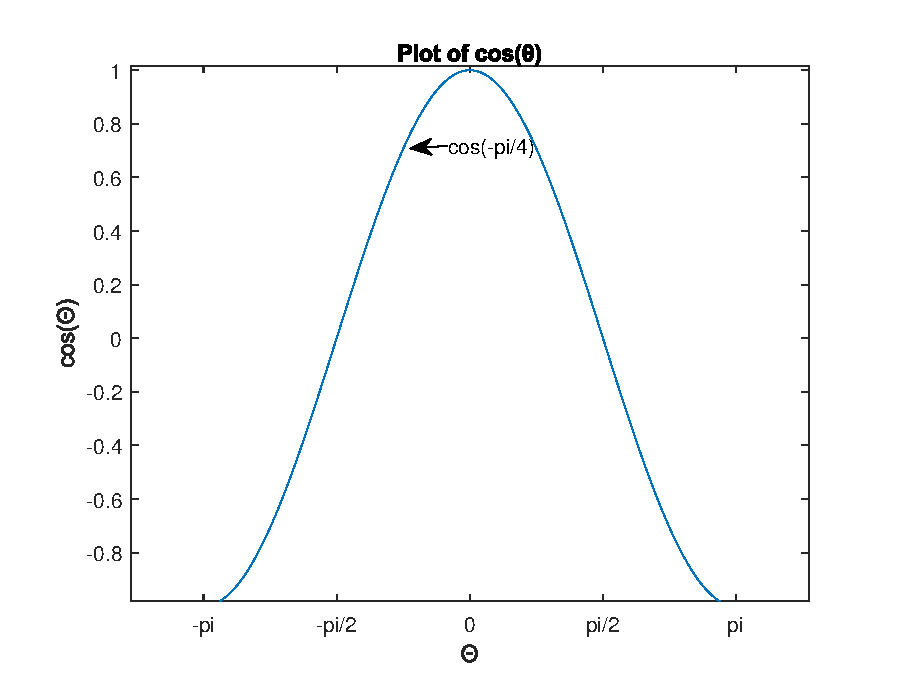
\includegraphics[width=10cm]{cosx.eps}\\
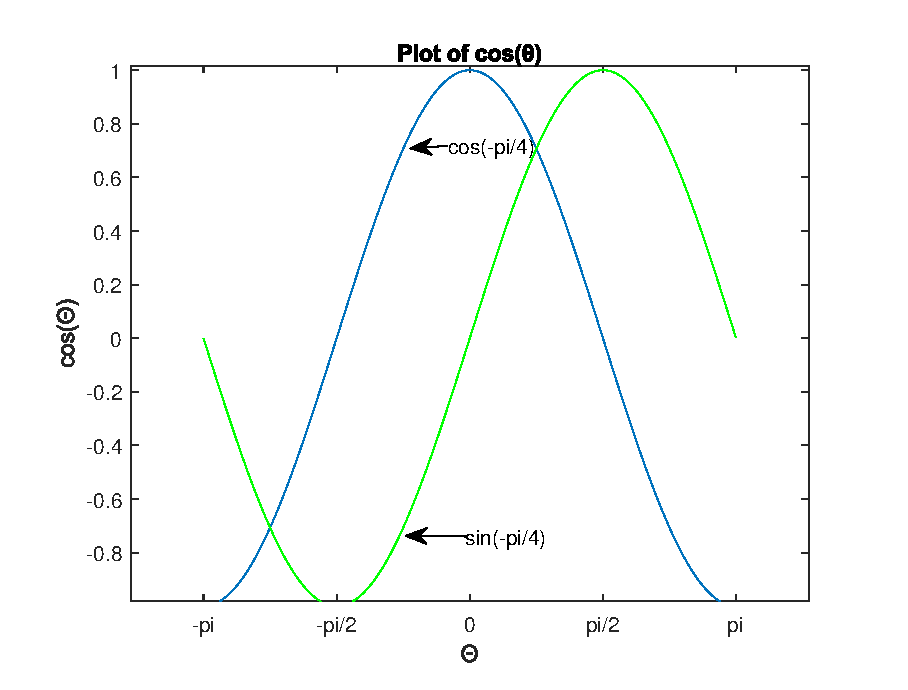
\includegraphics[width=10cm]{sinx.eps}
\end{center}



% =============================================================================== %
% ||                       HERE WE END OUR DOCUMENT                          || %
% =============================================================================== %
\end{document}
